\documentclass[10pt,letterpaper]{article}

% The visual and typographic system follows the supplied two-column template.
\usepackage[T1]{fontenc}
\usepackage{amsmath,amssymb,amsthm,mathtools}
\usepackage{newtxtext,newtxmath}
\usepackage{bm}
\usepackage[letterpaper,top=0.78in,bottom=0.80in,left=0.72in,right=0.72in,headheight=13pt,headsep=0.20in,footskip=0.37in]{geometry}
\setlength{\columnsep}{0.28in}
\setlength{\columnseprule}{0pt}
\usepackage{microtype}
\usepackage{xcolor}
\definecolor{VelvetBlue}{HTML}{000D3C}
\definecolor{MutedInk}{HTML}{525864}
\definecolor{TrendOrange}{HTML}{B75A3C}
\definecolor{MeanGreen}{HTML}{257A62}
\usepackage{booktabs,needspace}
\usepackage{dblfloatfix}
\usepackage{enumitem}
\usepackage{titlesec}
\usepackage{fancyhdr}
\usepackage{caption}
\usepackage{tikz}
\usetikzlibrary{arrows.meta,positioning,calc}
\usepackage{pgfplots}
\pgfplotsset{compat=1.18}
\usepackage[colorlinks=true,linkcolor=VelvetBlue,urlcolor=VelvetBlue,citecolor=VelvetBlue]{hyperref}
\hypersetup{pdftitle={From Max-Cut to Semidefinite Relaxation, EVA, and Clustering-Based Rounding},pdfauthor={maxkcut research tutorial},pdfsubject={An introductory guide to Max-Cut, SDP, EVA, random hyperplanes, and spherical k-means rounding}}
\titleformat{\section}[hang]
  {\color{VelvetBlue}\normalsize\bfseries}
  {\thesection}{0.75em}{}
  [\vspace{.26ex}{\color{VelvetBlue!23}\titlerule[0.35pt]}]
\titlespacing*{\section}{0pt}{2.6ex plus .7ex minus .2ex}{1.0ex}
\titleformat{\subsection}[hang]
  {\color{VelvetBlue}\normalsize\bfseries}
  {\thesubsection}{0.7em}{}
\titlespacing*{\subsection}{0pt}{2.0ex plus .4ex minus .2ex}{0.7ex}
\titleformat{\paragraph}[runin]
  {\normalfont\bfseries\color{VelvetBlue}}
  {}{0pt}{}
\titlespacing*{\paragraph}{0pt}{1.6ex plus .4ex minus .2ex}{0.65em}
\fancyhf{}
\fancyhead[L]{\scriptsize\textcolor{MutedInk}{MAX-CUT, SDP, EVA \& ROUNDING}}
\fancyhead[R]{\scriptsize\textcolor{VelvetBlue}{INTRODUCTORY TUTORIAL}}
\fancyfoot[C]{\footnotesize\textcolor{MutedInk}{\thepage}}
\renewcommand{\headrulewidth}{0.35pt}
\renewcommand{\footrulewidth}{0pt}
\pagestyle{fancy}
\fancypagestyle{firstpage}{\fancyhf{}\fancyfoot[C]{\footnotesize\textcolor{MutedInk}{\thepage}}\renewcommand{\headrulewidth}{0pt}}
\captionsetup{font=footnotesize,labelfont={bf,color=VelvetBlue},labelsep=period,skip=5pt}
\setlength{\parindent}{1.05em}
\setlength{\parskip}{0pt plus .3pt}
\setlength{\abovedisplayskip}{7pt plus 2pt minus 2pt}
\setlength{\belowdisplayskip}{7pt plus 2pt minus 2pt}
\setlength{\abovedisplayshortskip}{4pt plus 2pt minus 1pt}
\setlength{\belowdisplayshortskip}{5pt plus 2pt minus 2pt}
\setlist[enumerate]{topsep=5pt,itemsep=3pt,parsep=0pt,leftmargin=2em}
\setlist[itemize]{topsep=4pt,itemsep=2pt,parsep=0pt,leftmargin=1.5em}
\renewcommand{\arraystretch}{1.13}
\newcommand{\R}{\mathbb{R}}
\newcommand{\norm}[1]{\left\lVert#1\right\rVert}
\newcommand{\ip}[2]{\left\langle#1,#2\right\rangle}
\DeclareMathOperator{\diag}{diag}
\DeclareMathOperator{\Tr}{Tr}
\DeclareMathOperator{\rank}{rank}
\newcommand{\I}{\mathbf 1}
\newcommand{\explain}[1]{{\color{MeanGreen}\textbf{#1}}}

\begin{document}
\twocolumn[{\begin{@twocolumnfalse}
\thispagestyle{firstpage}
\noindent{\sffamily\color{VelvetBlue}\bfseries\scriptsize MATHEMATICAL TUTORIAL \enspace/\enspace MAXKCUT RESEARCH PROJECT}
\par\vspace{0.75em}
\noindent{\fontsize{19}{23}\selectfont\bfseries\color{VelvetBlue}
From Max-Cut to Semidefinite Programming,\\[2pt]
EVA, and Clustering-Based Rounding\par}
\vspace{0.8em}
\noindent{\color{MutedInk}\itshape A step-by-step introduction, from graphs and matrices to reproducible G-set experiments\par}
\vspace{0.9em}
\noindent{\color{VelvetBlue!30}\rule{\linewidth}{0.6pt}}
\vspace{0.45em}
\begingroup\small
\noindent{\color{VelvetBlue}\bfseries Abstract}\par\vspace{0.35em}
\noindent
\emph{Max-Cut} asks how to split the vertices of a weighted graph into two groups so that the total weight of the edges crossing between them is as large as possible. Searching over all splits is generally intractable. We build the problem from first principles, reformulate it using signs and matrices, and derive a \emph{semidefinite programming} (SDP) relaxation. We then explain the geometry of unit vectors, how the nonconvex \emph{Efficient Vector Ascent} (EVA) algorithm optimizes a low-rank factor of the SDP variable, and how three different rounding methods---Goemans--Williamson random hyperplanes, K-Means2N, and K-MeansNM---convert continuous vectors into an actual graph partition. We conclude with the G-set benchmark, convergence and precision, independent random restarts, and an exact description of the project's saved-factor workflow. All formulae concern \emph{Max-Cut} ($k=2$), with the distinction from general Max-$k$-Cut stated explicitly.
\par\endgroup\vspace{1.1em}
\end{@twocolumnfalse}}]

\section{What are we trying to solve?}
\label{sec:goal}
\paragraph{Graphs.} A \emph{graph} is a set of vertices (objects) joined by edges (relationships). Write
\begin{equation}
 G=(V,E,w),\qquad V=\{1,\ldots,n\}.
\end{equation}
Here $E$ contains pairs $\{i,j\}$ of vertices; $w_{ij}=w_{ji}\in\R$ is the weight of their edge, and we use $w_{ij}=0$ when no edge exists. We exclude self-loops, so $w_{ii}=0$.

\paragraph{A cut.} Divide $V$ into two groups $A$ and $V\setminus A$. An edge is \emph{cut} if its endpoints are in different groups. Its weight contributes to our score. The Max-Cut problem is
\begin{equation}\label{eq:cut-set}
 \max_{A\subseteq V} F(A),\qquad
 F(A)=\sum_{\substack{i<j\\\I[i\in A]\ne\I[j\in A]}}w_{ij}.
\end{equation}
The indicator $\I[P]$ equals $1$ when proposition $P$ is true, otherwise $0$.

\begin{figure}[t]
\centering
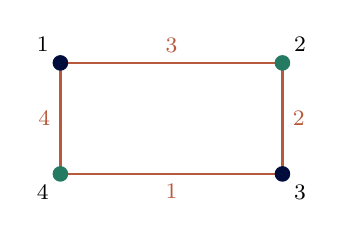
\begin{tikzpicture}[scale=.94,every node/.style={font=\footnotesize}]
\coordinate (a) at (0,1.5);\coordinate (b) at (3,1.5);
\coordinate (c) at (3,0);\coordinate (d) at (0,0);
\draw[thick,TrendOrange] (a)--node[above]{$3$}(b);
\draw[thick,TrendOrange] (b)--node[right]{$2$}(c);
\draw[thick,TrendOrange] (c)--node[below]{$1$}(d);
\draw[thick,TrendOrange] (d)--node[left]{$4$}(a);
\fill[VelvetBlue] (a) circle (3pt) (c) circle (3pt);
\fill[MeanGreen] (b) circle (3pt) (d) circle (3pt);
\node[above left=1pt] at (a) {$1$};\node[above right=1pt] at (b) {$2$};
\node[below right=1pt] at (c) {$3$};\node[below left=1pt] at (d) {$4$};
\end{tikzpicture}
\caption{A weighted four-cycle. The blue vertices $\{1,3\}$ and green vertices $\{2,4\}$ form a cut of weight $3+2+1+4=10$. Every edge crosses.}
\label{fig:cut}
\end{figure}

For the four-cycle in Figure~\ref{fig:cut}, choosing $A=\{1,3\}$ cuts all four edges. Choosing $A=\{1,2\}$ cuts only the edges of weight $2$ and $4$, scoring $6$. \emph{The objective measures crossing-edge weights, not geometric distances between graph vertices.}

\paragraph{Signed weights.} Some benchmark graphs have weights $+1$ or $-1$. Cutting a negative edge \emph{reduces} the objective: we prefer, when possible, to leave its endpoints in the same group. The optimization formula remains valid, but some classical approximation guarantees require \emph{nonnegative} weights.

\paragraph{Why is this hard?} There are $2^n$ sign assignments, but swapping the two groups does not change a cut. Thus there are $2^{n-1}$ distinct bipartitions. For large $n$ exhaustive search is unrealistic. General weighted Max-Cut is NP-hard: no known polynomial-time algorithm solves all instances exactly \cite{karp1972,goemans1995}.

\section{Replace sets by signs}
\label{sec:signs}
Assign every vertex a variable
\begin{equation}
 s_i=\begin{cases}+1,&i\in A,\\-1,&i\notin A.\end{cases}
 \qquad s\in\{-1,+1\}^n.
\end{equation}
The key algebraic trick is
\begin{equation}\label{eq:indicator}
 \I[s_i\ne s_j]=\frac{1-s_i s_j}{2}.
\end{equation}
Check both cases: equal signs yield $1-1=0$; opposite signs yield $1-(-1)=2$. Therefore
\begin{equation}\label{eq:iqp}
 \boxed{\max_{s\in\{-1,+1\}^n}
 \frac12\sum_{i<j}w_{ij}(1-s_is_j).}
\end{equation}
This is an \emph{integer quadratic optimization} problem. It is quadratic because pairs $s_is_j$ appear; it is discrete because every $s_i$ has only two possible values. If $C=\tfrac12\sum_{i<j}w_{ij}$, then
\begin{equation}\label{eq:spin-min}
 F(s)=C-\tfrac12\sum_{i<j}w_{ij}s_is_j.
\end{equation}
Thus maximizing the cut is \emph{equivalent} to
\begin{equation*}
 \min_{s\in\{-1,+1\}^n}\sum_{i<j}w_{ij}s_is_j.
\end{equation*}
Changing the objective to minimization does not make the discrete problem convex. The analogous continuous minimization is
\begin{equation*}
 \min_{\norm{y_i}=1\ \forall i}
 \sum_{i<j}w_{ij}y_i^\top y_j.
\end{equation*}


\paragraph{Tiny numerical example.} Take three vertices and edges $w_{12}=2$, $w_{23}=1$, $w_{13}=-1$. If $s=(1,-1,1)^\top$, edges $12$ and $23$ cross but edge $13$ does not. Hence $F(s)=2+1=3$. By Eq.~\eqref{eq:iqp},
\begin{equation*}
 \tfrac12[2(1-(-1))+1(1-(-1))
    -1(1-1)]=3.
\end{equation*}
We have already turned a combinatorial question into algebra.

\section{Why do matrices enter the story?}
\label{sec:matrix}
\paragraph{Adjacency matrix.} Place all edge weights into the symmetric matrix $W=(w_{ij})\in\R^{n\times n}$. For our three-vertex example,
\begin{equation}
 W=\begin{pmatrix}0&2&-1\\2&0&1\\-1&1&0\end{pmatrix}.
\end{equation}
Every row describes one vertex's weighted neighbors. Most large graphs are \emph{sparse}: each vertex is connected to relatively few others, so the project stores $W$ in compressed-sparse-row (CSR) format.

\paragraph{Graph Laplacian.} Let $D=\diag(W\bm1)$, with $\bm1$ the all-ones vector, and define
\begin{equation}\label{eq:lap}
 L=D-W.
\end{equation}
Then an exact identity is
\begin{equation}\label{eq:lap-energy}
 s^\top Ls=\sum_{i<j}w_{ij}(s_i-s_j)^2.
\end{equation}
For signs, $(s_i-s_j)^2$ is $4$ if cut and $0$ otherwise, so
\begin{equation}\label{eq:lap-maxcut}
 \boxed{F(s)=\tfrac14 s^\top Ls.}
\end{equation}
When all weights are nonnegative, $L$ is positive semidefinite. With \emph{negative} weights this need not be true; our later SDP formulation remains meaningful nevertheless.

\paragraph{A matrix of pairwise relationships.} Introduce
\begin{equation}\label{eq:spin-gram}
 X=ss^\top,\qquad X_{ij}=s_is_j.
\end{equation}
For the example $s=(1,-1,1)^\top$,
\begin{equation}
 X=\begin{pmatrix}1&-1&1\\-1&1&-1\\1&-1&1\end{pmatrix}.
\end{equation}
Its diagonal is all ones; an off-diagonal entry is $+1$ for vertices in the same group and $-1$ for vertices in opposite groups.

\paragraph{PSD: positive semidefinite.} We say a symmetric matrix $X$ is \emph{positive semidefinite} (PSD), written $X\succeq0$, if
\begin{equation}\label{eq:psd}
 z^\top Xz\ge0\quad\text{for every }z\in\R^n.
\end{equation}
For $X=ss^\top$, this follows immediately:
\begin{equation}
 z^\top Xz=z^\top ss^\top z=(s^\top z)^2\ge0.
\end{equation}
All eigenvalues of a PSD matrix are nonnegative. The matrix $ss^\top$ is PSD, has $X_{ii}=1$, and has \emph{rank one} (all columns are multiples of $s$).

\section{Relaxing the impossible search}
\label{sec:relax}
A \emph{relaxation} enlarges the feasible set: it drops a difficult restriction to obtain a problem easier to solve. Its best objective can be larger than the true Max-Cut optimum. Such a value is an \emph{upper bound} only if the relaxed problem is solved exactly or a valid numerical certificate is available.

In Eq.~\eqref{eq:spin-gram} the condition $X=ss^\top$ forces rank one and discrete off-diagonal entries. We \emph{drop} that condition, retaining the necessary properties $X\succeq0$ and $\diag(X)=\bm1$. This produces
\begin{equation}\label{eq:sdp}
 \boxed{\begin{aligned}
 \text{maximize}_{X\in\mathbb S^n}\quad&
 \frac12\sum_{i<j}w_{ij}(1-X_{ij})\\
 \text{subject to}\quad&X\succeq0,\\
 &X_{ii}=1\quad(i=1,\ldots,n).
 \end{aligned}}
\end{equation}
Here $\mathbb S^n$ is the space of real symmetric $n\times n$ matrices. Using Eq.~\eqref{eq:lap}, the same objective is $\tfrac14\Tr(LX)$, where $\Tr$ denotes the trace (sum of diagonal entries).

\subsection{What is an SDP?}
The abbreviation is \emph{semidefinite program} (SDP), \emph{not} ``SPD.'' An SDP optimizes a linear function of a matrix under linear constraints and a PSD constraint. In Eq.~\eqref{eq:sdp}, every feasible matrix represents a relaxed configuration of all vertex pairs.

\paragraph{Why is it convex?} A set is convex when every line segment between two of its points stays inside the set. If $X_1,X_2\succeq0$ and $0\le t\le1$, then for every $z$,
\begin{equation}
 z^\top[tX_1+(1-t)X_2]z
 =t z^\top X_1z+(1-t)z^\top X_2z\ge0.
\end{equation}
Thus the PSD cone is convex. Also, $\diag(tX_1+(1-t)X_2)=\bm1$ if both diagonals are $\bm1$. Finally, the objective is \emph{linear in $X$}, hence simultaneously convex and concave. Therefore, maximizing it over this convex feasible set is a convex optimization problem. It has no spurious local maxima in the \emph{matrix variable $X$}.

\paragraph{What is \emph{not} convex?} The original feasible set of signs is discrete; the rank-one condition is nonconvex. We discarded that restriction, so the SDP may produce a matrix with fractional entries such as $X_{12}=0.3$. That matrix is valid for the relaxation but is \emph{not yet a cut}.

\section{From an SDP matrix to unit vectors}
\label{sec:gram}
Every PSD matrix has a Gram factorization
\begin{equation}\label{eq:gram}
 X=YY^\top,\quad Y=\begin{pmatrix}
 y_1^\top\\\vdots\\y_n^\top
 \end{pmatrix}\in\R^{n\times p},
\end{equation}
with $p=\rank(X)$ (or more columns if desired). Its entries are inner products:
\begin{equation}\label{eq:dot}
 X_{ij}=y_i^\top y_j,
 \qquad X_{ii}=\norm{y_i}^2=1.
\end{equation}
Thus every vertex is a \emph{unit vector}, a point on the unit sphere in $\R^p$. The inner product has an angular interpretation:
\begin{equation}\label{eq:cos}
 y_i^\top y_j=\cos\theta_{ij}
 \quad\text{when}\quad\norm{y_i}=\norm{y_j}=1.
\end{equation}
If the two vectors point in nearly opposite directions ($\cos\theta\approx-1$), the relaxation favors cutting that edge when $w_{ij}>0$. For a negative edge, similar directions are often preferable.

\begin{figure}[t]
\centering
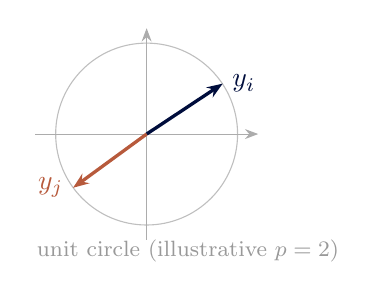
\begin{tikzpicture}[scale=1.05,>=Stealth]
\draw[gray!50] (0,0) circle (1.1);
\draw[->,gray!65] (-1.35,0)--(1.35,0);
\draw[->,gray!65] (0,-1.28)--(0,1.28);
\draw[-{Stealth[length=2mm]},very thick,VelvetBlue] (0,0)--(0.92,0.61);
\draw[-{Stealth[length=2mm]},very thick,TrendOrange] (0,0)--(-0.89,-0.65);
\node[VelvetBlue,right] at (0.92,0.61) {$y_i$};
\node[TrendOrange,left] at (-0.89,-0.65) {$y_j$};
\node[gray!80,font=\footnotesize] at (0.5,-1.41) {unit circle (illustrative $p=2$)};
\end{tikzpicture}
\caption{The SDP replaces signs by unit vectors. Opposite vectors have inner product near $-1$. Later we must map them back to discrete groups.}
\end{figure}

\paragraph{Why this helps.} Moving vectors continuously on a sphere provides many possible intermediate configurations, unlike the original two-valued signs. But until we perform \emph{rounding}, the vectors do not specify the final partition.

\section{The vector optimization and EVA}
\label{sec:eva}
Substituting Eq.~\eqref{eq:dot} into the SDP objective gives the \emph{vector relaxation}:
\begin{equation}\label{eq:vector}
 \boxed{\begin{aligned}
 \max_{y_1,\ldots,y_n\in\R^p}\quad&
 \Phi(Y)=\frac12\sum_{i<j}w_{ij}
 (1-y_i^\top y_j)\\
 \text{subject to}\quad&\norm{y_i}=1\ \forall i.
 \end{aligned}}
\end{equation}
If $p$ is unrestricted, it represents the full SDP Gram geometry. In our scalable experiments, $p\ll n$, reducing storage dramatically. But Eq.~\eqref{eq:vector} is \emph{nonconvex in $Y$}: the equality constraints $\norm{y_i}=1$ define spheres, and the objective contains products of vector coordinates.

\paragraph{The distinction in one sentence.} The \emph{full SDP} optimizes a large convex matrix $X$; \emph{EVA} optimizes a smaller, nonconvex factor $Y$. Both use the same continuous Max-Cut objective after applying $X=YY^\top$, but they solve different numerical formulations \cite{eva2026}.

\subsection{EVA means Efficient Vector Ascent}
EVA is a greedy \emph{block coordinate-ascent} algorithm: it optimizes one vertex vector at a time while holding all other vectors fixed. We can derive its update with just algebra.

For vertex $i$, define its weighted neighbor field
\begin{equation}\label{eq:field}
 h_i=\sum_{j:\{i,j\}\in E}w_{ij}y_j.
\end{equation}
Of the full objective, the terms that depend on $y_i$ are
\begin{equation}\label{eq:local}
 \Phi_i(y_i)=\text{constant}-\tfrac12 y_i^\top h_i.
\end{equation}
Hence maximizing $\Phi_i$ is equivalent to
\begin{equation}\label{eq:local-min}
 \min_{\norm{y_i}=1}y_i^\top h_i.
\end{equation}
By Cauchy--Schwarz, $y_i^\top h_i\ge-\norm{h_i}$; equality is attained by pointing $y_i$ directly \emph{against} $h_i$. Therefore
\begin{equation}\label{eq:eva-update}
 \boxed{y_i\gets-\frac{h_i}{\norm{h_i}}\quad(h_i\ne0).}
\end{equation}
If $h_i=0$, this vertex has no directional preference at that moment; our implementation draws a fresh random unit vector. This derivation is the heart of EVA.

\subsection{One complete sweep, step by step}
\label{sec:evasweep}
\begin{enumerate}
\item Choose an embedding dimension $p$. In our EVA implementation, independently sample all $p$ coordinates of each initial vector from $U(0,1)$, then normalize each row to have Euclidean norm one. (The later rounding directions use Gaussian sampling.)
\item Visit vertices in order $i=1,2,\ldots,n$.
\item Compute $h_i$ from \emph{current} neighbor vectors. Updates to earlier vertices in this sweep are already reflected.
\item Replace $y_i$ using Eq.~\eqref{eq:eva-update}; continue to the next vertex.
\item Measure the largest angular change, compute or audit the objective, and decide whether to stop.
\item If not converged, begin another sweep from vertex $1$.
\end{enumerate}
The update order matters computationally: a \emph{sequential} sweep is not the same as simultaneously replacing every vector using its old neighbors. Our accelerated Numba implementation compiles this loop while retaining the sequential method.

\paragraph{Why does one update help?} Let $y_i^{\rm old}$ and $y_i^{\rm new}$ be unit vectors, and $\theta_i$ the angle between them. The exact local improvement is
\begin{equation}\label{eq:gain}
 \begin{aligned}
 \Delta\Phi_i
 &=\tfrac12\bigl[(y_i^{\rm old})^\top h_i
      -(y_i^{\rm new})^\top h_i\bigr]\\
 &=\tfrac12\norm{h_i}(1-\cos\theta_i)\ge0.
 \end{aligned}
\end{equation}
So an exact nonzero-field update never decreases the continuous objective. We may accumulate these gains incrementally instead of rescanning all edges on every sweep. A numerical implementation should also check this against independently recomputed objectives periodically.

\subsection{When does EVA stop?}
Let $\theta_i^{(t)}$ denote the angular movement of vertex $i$ during sweep $t$. We stop when
\begin{equation}\label{eq:stop}
 \boxed{\max_i\theta_i^{(t)}<\varepsilon,\qquad
 \theta_i^{(t)}=\arccos\!\left(
 (y_i^{\rm old})^\top y_i^{\rm new}\right).}
\end{equation}
The argument to $\arccos$ is clipped to $[-1,1]$ to handle floating-point roundoff. The tolerance $\varepsilon$ is an \emph{angle in radians}, not a bound on the objective error or the distance to the globally optimal cut. We also specify a maximum number of sweeps. Reaching that cap is a different status from numerical convergence.

\paragraph{How precise should $\varepsilon$ be?} The original experiment used $10^{-3}$; the high-precision follow-up tests $10^{-6}$. Lower tolerance means a stricter stopping test, potentially many more sweeps, not necessarily a better discrete cut. Near $\theta=0$, $\arccos(1-\delta)$ is sensitive to floating-point rounding. An extreme target such as $10^{-12}$ is generally not reliable under a naive double-precision angle test.

\subsection{Rank, efficiency, and guarantees}
A common default in the EVA study and our repository is
\begin{equation}\label{eq:rank}
 p=\left\lceil\sqrt{2(n+1)}\right\rceil.
\end{equation}
For $n=800$, $p=41$; for $n=20{,}000$, $p=201$. The factor $Y$ needs $np$ floating-point numbers; the dense $X$ needs $n^2$. At $n=20{,}000$ in float64, the raw factor is about $32.2$~MB while a single dense Gram matrix occupies about $3.2$~GB (decimal units). A complete general-purpose SDP solver may need much more memory than one Gram matrix.

EVA performs a sparse weighted neighbor aggregation for each vertex, giving approximately $O(mp)$ arithmetic per sweep, where $m=|E|$, and $O(m+np)$ sparse-graph-plus-factor memory. Low-rank Burer--Monteiro theory gives useful relationships between rank, stationarity, and SDP optima \cite{eva2026,burer2003}; however, a particular stopped, nonconvex numerical run is \emph{not} a certified globally optimal SDP solve. Likewise, a high continuous value is not proof of an optimal discrete cut.

\section{What exactly is rounding?}
\label{sec:round}
A continuous vector solution $Y$ may contain real numbers, but Max-Cut requires exactly two groups. \emph{Rounding} is any rule that converts the row vectors $y_1,\ldots,y_n$ into a label $c_i\in\{0,1\}$ or sign $s_i\in\{-1,1\}$ for every vertex.

The actual cut value of the resulting partition is evaluated on the \emph{original graph}:
\begin{equation}\label{eq:rounded-score}
 F(c)=\sum_{i<j}w_{ij}\I[c_i\ne c_j].
\end{equation}
This is not the same as the continuous objective $\Phi(Y)$. Because rounding loses information, two methods applied to the \emph{same} $Y$ can find different cuts.

\paragraph{A stochastic algorithm.} An algorithm is \emph{randomized} when it samples internal random values. One execution is a \emph{trial} or \emph{restart}. Repeating it with independent seeded random choices may produce a different partition. The core question of this work is whether clustering the vectors can outperform a single random separating hyperplane \cite{rodriguez2020,thesis2021}.

\section{Method 1: the original random hyperplane}
\label{sec:gw}
\paragraph{Goemans--Williamson (GW).} This is the classic randomized rounding method for Max-Cut \cite{goemans1995}. It is called \texttt{FJ\_EVA} in our saved EVA experiments for consistency with a more general rounding interface; \emph{for $k=2$ it is GW}, not a new random algorithm.

\begin{enumerate}
\item Start with the \emph{fixed}, saved matrix $Y\in\R^{n\times p}$.
\item Draw a random direction $r\in\R^p$ by sampling each coordinate from a standard normal distribution $\mathcal N(0,1)$.
\item For each vertex compute the scalar projection $q_i=y_i^\top r$.
\item Assign $c_i=1$ when $q_i\ge0$, and $c_i=0$ otherwise.
\item Compute $F(c)$ from Eq.~\eqref{eq:rounded-score}; save the partition and score.
\end{enumerate}
Equivalently,
\begin{equation}\label{eq:gw}
 c_i=\I[y_i^\top r\ge0].
\end{equation}
For example, with $p=2$, $y_1=(1,0)$, $y_2=(-1,0)$, and random direction $r=(2,1)$, we obtain $q_1=2$ and $q_2=-2$, hence different groups. If their edge weight is $3$, this edge contributes $3$ to the resulting cut. Another draw of $r$ can change assignments of other vertices.

The hyperplane perpendicular to $r$ and passing through the origin separates the sphere into two hemispheres. Two vectors with angle $\theta_{ij}$ are separated with probability
\begin{equation}\label{eq:gwprob}
 \Pr(c_i\ne c_j)=\frac{\theta_{ij}}{\pi}.
\end{equation}
For graphs with nonnegative weights and a suitably solved SDP, GW's celebrated expected approximation ratio is at least about $0.87856$ of the true Max-Cut optimum \cite{goemans1995}. \emph{This statement must not be transferred without qualification to signed-weight G-set instances or arbitrary nonconvex EVA factors.}

\begin{figure}[t]
\centering
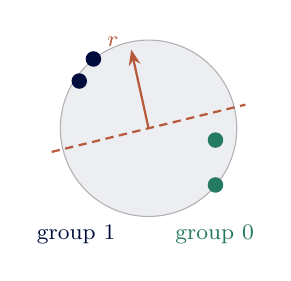
\begin{tikzpicture}[scale=1.0]
\fill[VelvetBlue!7] (0,0) circle (1.12);
\draw[gray!60] (0,0) circle (1.12);
\draw[densely dashed,TrendOrange,thick] (-1.23,-.30)--(1.23,.30);
\fill[VelvetBlue] (-.70,.88) circle (2.8pt) (-.88,.60) circle (2.8pt);
\fill[MeanGreen] (.85,-.72) circle (2.8pt) (.85,-.15) circle (2.8pt);
\draw[-{Stealth[length=2mm]},thick,TrendOrange] (0,0)--(-.22,1.0);
\node[font=\footnotesize,TrendOrange] at (-.45,1.1) {$r$};
\node[font=\footnotesize,VelvetBlue] at (-.92,-1.35) {group $1$};
\node[font=\footnotesize,MeanGreen] at (.84,-1.35) {group $0$};
\end{tikzpicture}
\caption{The random direction $r$ defines a perpendicular separating line in $p=2$; in higher dimensions it defines a hyperplane. Each side becomes a cut group.}
\end{figure}

\section{Method 2: K-Means2N}
\label{sec:2n}
\paragraph{Clustering.} A \emph{cluster} is a collection of similar vectors. In $k$-means, each cluster is represented by a center (\emph{centroid}), and each point is repeatedly assigned to the nearest center. Here $k=2$ is the \emph{number of clusters}, not the embedding dimension $p$.

Because our vectors all have length one, we use \emph{spherical $k$-means}. Each centroid is normalized after updating. For unit vectors $u,v$,
\begin{equation}\label{eq:cos-vs-distance}
 \norm{u-v}^2=2(1-u^\top v),
\end{equation}
so maximizing cosine similarity $u^\top v$ is equivalent to minimizing Euclidean distance between normalized vectors \cite{rodriguez2020}.

\subsection{Algorithm, step by step}
\begin{enumerate}
\item Sample two \emph{independent} Gaussian vectors $r_1,r_2\in\R^p$.
\item Normalize them: $\mu_j=r_j/\norm{r_j}$ for $j=1,2$.
\item Assign each vertex to the center having the larger inner product:
\begin{equation}\label{eq:assign}
 c_i\gets\arg\max_{j\in\{1,2\}}
 y_i^\top\mu_j.
\end{equation}
\item For each cluster, sum its member vectors and normalize:
\begin{equation}\label{eq:centroid}
 \mu_j\gets\frac{\sum_{i:c_i=j}y_i}
 {\left\|\sum_{i:c_i=j}y_i\right\|}.
\end{equation}
\item Repeat assignment and centroid updates until labels stop changing or 100 iterations have been attempted.
\item Return the resulting labels; score the partition on the original weighted graph.
\end{enumerate}
In the implementation, empty or zero-sum clusters receive a randomly chosen data-vector center. The \emph{two independent initial directions} distinguish K-Means2N from K-MeansNM.

\paragraph{What $k$-means optimizes.} It makes vectors compact around their centroids (equivalently, increases total within-cluster cosine similarity). It does \emph{not} directly optimize the graph cut $F(c)$. An improvement in clustering compactness may or may not improve the cut. K-Means2N has no universal guarantee of outperforming a paired GW cut \cite{rodriguez2020}.

\section{Method 3: K-MeansNM}
\label{sec:nm}
K-MeansNM is also spherical $2$-means, but its \emph{initialization and selection} are different. The method uses an \emph{antipodal initialization}: the second initial direction is the negative of the first.

\begin{enumerate}
\item Draw one Gaussian direction $r\in\R^p$ and normalize it.
\item Initialize opposite centroids:
\begin{equation}\label{eq:antipodal}
 \mu_1=\frac{r}{\norm{r}},\qquad
 \mu_2=-\mu_1.
\end{equation}
\item Assign each vertex by Eq.~\eqref{eq:assign}. Because the centers are opposite, this is exactly the same initial bipartition as a GW hyperplane with direction $r$ (up to label names and zero ties).
\item Calculate the actual weighted cut $F(c)$ and store the best labels seen so far.
\item Perform the spherical centroid updates and reassignments as in K-Means2N. After \emph{every assignment}, recompute $F(c)$ and retain it if it is better than the saved best.
\item Stop at stable labels or the iteration limit; return the \emph{best encountered cut}, possibly from an intermediate iteration rather than the final clustering assignment.
\end{enumerate}

\paragraph{Why retaining the initial cut matters.} The first assignment is a valid GW cut. Since our implementation saves the maximum $F(c)$ over the initial and subsequent assignments,
\begin{equation}\label{eq:nm-monotone}
 F_{\rm NM,kept}\ge F_{\rm GW,paired}.
\end{equation}
This is a \emph{per-trial implementation guarantee} for the same Gaussian direction $r$; it is not a proof that $k$-means clustering monotonically increases the cut at every iteration. Clustering can temporarily worsen it, and Eq.~\eqref{eq:nm-monotone} does not establish a better worst-case approximation ratio for arbitrary signed-weight graphs.

\paragraph{A controlled comparison.} In the repository, GW and K-MeansNM use matched initial random directions for the same graph and restart index. Thus one can compare the two starting from a common hyperplane. K-Means2N uses two independent random directions and a different random stream. All three are still evaluated using the exact same graph and continuous factor $Y$.

\section{Why not round just once?}
\label{sec:restarts}
Consider one expensive continuous optimization producing $Y$. The graph and the vector factor now remain \emph{fixed}. Randomized hyperplanes and randomized centroid initializations may yield different partitions on different trials. Therefore we can run the \emph{cheap rounding stage many times} without solving another SDP or running EVA again.

\paragraph{What a restart means here.} One rounding restart is one new draw of the random direction(s), followed by the relevant clustering updates and one saved partition. It is \emph{not} a new EVA run, a new graph, or a new SDP solve. With $R$ restarts per method and three methods, we obtain $3R$ candidate cuts per graph from the same $Y$.

\begin{equation}\label{eq:trialcounts}
 \begin{aligned}
 R=20&:\quad60\ \text{cuts per graph},\\
 R=100&:\quad300\ \text{cuts per graph},\\
 R=1{,}000&:\quad3{,}000\ \text{cuts per graph}.
 \end{aligned}
\end{equation}
For 71 graphs, 1,000 trials of each of three methods would yield 213,000 candidate cuts \emph{if every graph has a completed factor}. These trials improve our \emph{search among discrete cuts}; they do not change the fixed continuous objective $\Phi(Y)$.

\paragraph{Why keep all scores?} Reporting only the largest cut can hide variability. For scores $F_1,\ldots,F_R$, report at least
\begin{equation}
 \bar F=\frac1R\sum_{r=1}^RF_r,
 \quad F_{\max}=\max_{1\le r\le R}F_r,
\end{equation}
and preferably their median, standard deviation, trial count, seed, and factor identity. A method may have a high best cut but unstable typical performance.

\paragraph{A probability illustration.} If (hypothetically) each independent trial has probability $q$ of finding a specified quality threshold, the chance of finding it at least once in $R$ independent trials is
\begin{equation}\label{eq:repeated}
 1-(1-q)^R.
\end{equation}
This is why more restarts can help. But restarts from the \emph{same factor} are not independent graph instances. They may share biases and cannot fix a poor continuous factor automatically.

\section{What are the G-set graphs?}
\label{sec:gset}
The \emph{G-set} is a widely used benchmark collection of weighted Max-Cut graphs created using Rinaldi's graph generator and distributed through Y. Ye's resource. It includes toroidal, nearly planar, and random graph topologies. The canonical collection used in this project has 71 instances:
\begin{equation}\label{eq:gset-ids}
 \{\mathrm{G1},\ldots,\mathrm{G67},
 \mathrm{G70},\mathrm{G72},\mathrm{G77},\mathrm{G81}\}.
\end{equation}
They contain approximately 800 to 20,000 vertices with edge weights $\pm1$ \cite{rodriguez2020,thesis2021}.

\paragraph{Why is G-set famous?} Researchers need common test problems to compare algorithms. If several papers use the same named graph and scoring convention, one can compare the best attained cut, convergence, memory, and run time. Many instances have no proven discrete optimum, so a published \emph{best-known cut} is not automatically a mathematical optimum.

\paragraph{Historical context.} The 2020 clustering paper and 2021 dissertation report that their full-SDP tools could not solve several large instances, including G55, G56, G60, G61, G70, G77, and G81 \cite{rodriguez2020,thesis2021}. That is an observation about their solver/resources, \emph{not} a proof these graphs cannot be processed by other algorithms. EVA's factor representation makes such larger instances much more practical.

\paragraph{Why exact input identity matters.} Two files with the same graph name may differ in format, edge ordering, or weights. Our repository uses the canonical \,\texttt{data/G*.txt}\, files and records a SHA256 hash of each input. A valid comparison must refer to the same \emph{weighted} graph and objective convention.

\section{SDP once, rounding many times}
\label{sec:workflow}
\paragraph{The essential pipeline.} The large optimization problem is solved once for a \emph{fixed graph, formulation, seed, rank and tolerance}; then the saved continuous vectors are reused for independently randomized rounding trials:
\begin{equation}\label{eq:pipeline}
 \underbrace{G\longrightarrow Y}_{\substack{\text{EVA once}\\\text{for fixed settings}}}
 \ \longrightarrow\ 
 \underbrace{c^{(1)},\ldots,c^{(R)}}_{\text{round many times}}
 \longrightarrow\ F(c^{(r)}).
\end{equation}
The conventional convex-SDP route is $G\to X\succeq0\to Y\to$ rounding. The EVA route is $G\to Y\to$ rounding; \emph{EVA never needs to form the dense $X$ explicitly}. If we change the graph, EVA rank, optimization seed, or convergence tolerance, we have a \emph{new optimization experiment} and should not silently reuse an incompatible checkpoint.

\paragraph{What is saved in the project?} The project's EVA command writes a per-graph factor archive \,\texttt{factors/Gxx.npz}\, containing all vectors $Y$, convergence metadata and RNG state; \,\texttt{logs/Gxx-sweeps.jsonl}\, for the optimization trajectory; \,\texttt{cases/Gxx.json}\, for summary and provenance; and a verified partition archive with each method's individual labels and scores. A separate \texttt{eva\_rounding\_cli} can append nonoverlapping restart-index ranges using the \emph{same verified factor}, while keeping exact snapshots and hashes.

\paragraph{Why hashes and checkpoints?} They make it possible to verify that a later rounding batch really used the intended graph and vectors and that the optimization can resume after interruption. One should never mix scores from different factor versions as if they came from the same continuous solution.

\paragraph{Two meanings of ``solve''.} A completed \emph{EVA solve} means the continuous factor optimizer converged according to Eq.~\eqref{eq:stop} or reached its cap. A completed \emph{rounding trial} means it produced a valid binary partition and an exact weighted cut value. Neither event alone establishes the globally optimal discrete Max-Cut value.

\section{Optional: local search after rounding}
\label{sec:flips}
The repository also supports \emph{one-vertex-flip local search} as an additional postprocessing step. Starting from any rounded sign vector $s$, flip one sign $s_i\gets-s_i$ if doing so improves the cut. The exact gain is
\begin{equation}\label{eq:flipgain}
 \Delta_i F=s_i\sum_jw_{ij}s_j.
\end{equation}
To derive it, only edges adjacent to $i$ change their contribution. Accepting only positive gains guarantees that each accepted flip increases the actual cut. Repeat until no improving flip is found or the sweep budget is exhausted. The saved methods \texttt{FJ-Flip\_EVA} and \texttt{K-MeansNM-Flip\_EVA} apply this to their corresponding initial rounding results. This is a \emph{local heuristic}, not an exact Max-Cut solver.

\section{What changes for Max-\texorpdfstring{$k$}{k}-Cut?}
\label{sec:maxk}
Everything above has concentrated on $k=2$: two groups, one sign per vertex. For Max-$k$-Cut, we partition vertices into \emph{$k$} groups ($k\ge2$), and the discrete objective is still the weight of edges whose endpoints have different labels.

An important SDP relaxation for Max-$k$-Cut is the Frieze--Jerrum program
\begin{equation}\label{eq:frieze-jerrum}
 \begin{aligned}
 \max_{X\succeq0}\quad&\frac{k-1}{2k}\Tr(LX)\\
 \text{subject to}\quad& X_{ii}=1\ \forall i,\\
 &X_{ij}\ge-\frac1{k-1}\ \forall i\ne j.
 \end{aligned}
\end{equation}
At $k=2$, the lower bound is $-1$, which follows automatically from PSD and unit diagonal; Eq.~\eqref{eq:sdp} is recovered. For $k>2$, that additional constraint is generally essential. One can use $k$ Gaussian directions for a corresponding randomized rounding step, but the binary EVA implementation and the three named two-cluster methods in this tutorial \emph{do not by themselves solve the general Max-$k$-Cut SDP}. See \cite{friezejerrum1997,jmlr2022} for broader perspectives.

\section{How should we judge an experiment?}
\label{sec:judgement}
\begin{enumerate}
\item \explain{Verify the input.} Record graph name, vertex and edge counts, weights and SHA256.
\item \explain{Describe the optimizer.} Say whether $Y$ came from Numba EVA, NumPy EVA, or a factorization of convex-SDP output; report rank, tolerance, seed, sweeps and timing.
\item \explain{Separate objectives.} Report the continuous $\Phi(Y)$ and the actual integer $F(c)$ separately. Do not call the first an attained discrete cut.
\item \explain{Specify all rounding budgets.} Each method should have named seeds, restart indices, number of trials and a reproducible partition archive.
\item \explain{Compare fairly.} Use the same saved factor when isolating the effect of GW versus K-Means2N versus K-MeansNM. Changing the optimizer and rounder simultaneously confounds the comparison.
\item \explain{Measure more than the best.} Report best, mean, median, dispersion and paired differences when methods share the initial hyperplane.
\item \explain{Be careful with guarantees.} For signed graphs, do not assume the nonnegative-weight GW $0.87856$ theorem applies. Numerically approximate SDP primal objectives are not automatically certified bounds.
\end{enumerate}

\section{A complete mental picture}
\label{sec:summary}
We began with a graph whose vertices must be separated into two groups. Signs made the cut objective algebraic. A rank-one matrix $ss^\top$ encoded those signs, but the rank restriction was difficult. Dropping it produced a convex SDP over PSD matrices. Such matrices can be represented as inner products of unit vectors. EVA works directly with a low-rank collection of those vectors and repeatedly optimizes one vector at a time, using a simple closed-form update. Finally, randomized rounding or spherical clustering converts the continuous vectors back to actual binary graph partitions.

\begin{center}
\small\color{VelvetBlue}\bfseries
Graph $\to$ signs $\to$ Gram matrix $\to$\newline
SDP/vector relaxation $\to$ EVA factor $Y$ $\to$\newline
GW / K-Means2N / K-MeansNM $\to$ cut.
\end{center}

The key experimental economy is that \emph{the expensive continuous solution can be reused}. Thousands of rounding trials explore many cuts with a fixed factor, while changes in EVA tolerance or rank require a separately identified continuous experiment.

\section*{Glossary}
\addcontentsline{toc}{section}{Glossary}
\begin{description}[leftmargin=0pt,labelindent=0pt,style=nextline,itemsep=2pt,parsep=0pt]
\item[Cut] A partition of graph vertices into two sets.
\item[Objective] The number or expression we maximize or minimize.
\item[Relaxation] A larger feasible set that simplifies optimization.
\item[PSD] A symmetric matrix with $z^\top Xz\ge0$ for every $z$.
\item[SDP] A semidefinite program: linear matrix optimization with PSD constraints.
\item[Gram matrix] A matrix of pairwise inner products $X_{ij}=y_i^\top y_j$.
\item[Embedding dimension] The number $p$ of coordinates per vector.
\item[EVA sweep] One sequential visit through all vertex vectors.
\item[Rounding] Turning continuous vectors into discrete labels.
\item[Centroid] A representative direction of a cluster.
\item[Restart] A new random rounding initialization on a fixed factor.
\item[Convergence tolerance] A threshold on numerical change; not a global optimality guarantee.
\end{description}

\section*{Sources and further reading}
\addcontentsline{toc}{section}{Sources and further reading}
\begin{thebibliography}{99}\setlength{\itemsep}{2pt}
\bibitem{goemans1995} M.~X. Goemans and D.~P. Williamson (1995). Improved approximation algorithms for maximum cut and satisfiability problems using semidefinite programming. \emph{J. ACM} 42(6), 1115--1145. \url{https://doi.org/10.1145/227683.227684}.
\bibitem{rodriguez2020} A.~E. Rodr\'iguez-Fern\'andez, B. Gonz\'alez-Torres, R. Menchaca-M\'endez, and P.~F. Stadler (2020). Clustering improves the Goemans--Williamson approximation for the Max-Cut problem. \emph{Computation} 8(3), 75. \url{https://doi.org/10.3390/computation8030075}.
\bibitem{thesis2021} A.~E. Rodr\'iguez Fern\'andez (2021). \emph{On the Study of Fitness Landscapes and the Max-Cut Problem}. Doctoral dissertation, Leipzig University, especially Chapter 6. (User-provided thesis.)
\bibitem{eva2026} B. Gonz\'alez-Torres, A.~E. Rodr\'iguez-Fern\'andez, R. Menchaca-M\'endez, R. Menchaca-M\'endez, and O. Sch\"utze (2026). EVA: A fast greedy optimization algorithm for the Max-Cut vector relaxation problem. \emph{Results in Control and Optimization} 24, 100759. \url{https://doi.org/10.1016/j.rico.2026.100759}. Original MATLAB code: \url{https://github.com/b3r8/EVA}.
\bibitem{burer2003} S. Burer and R.~D.~C. Monteiro (2003). A nonlinear programming algorithm for solving semidefinite programs via low-rank factorization. \emph{Mathematical Programming} 95, 329--357. \url{https://doi.org/10.1007/s10107-002-0352-8}.
\bibitem{friezejerrum1997} A. Frieze and M. Jerrum (1997). Improved approximation algorithms for MAX $k$-CUT and MAX BISECTION. \emph{Algorithmica} 18, 67--81. \url{https://doi.org/10.1007/BF02523688}.
\bibitem{jmlr2022} P. Felzenszwalb, C. Klivans, and A. Paul (2022). Clustering with semidefinite programming and fixed point iteration. \emph{J. Mach. Learn. Res.} 23, paper 21-0402. \url{https://jmlr.org/papers/v23/21-0402.html}.
\bibitem{karp1972} R.~M. Karp (1972). Reducibility among combinatorial problems. In \emph{Complexity of Computer Computations}, 85--103.
\end{thebibliography}
\end{document}